% artigo científico escrito por Tatiana Balbi Fraga
% incluir texto apresentando o trabalho

%%%%%%%%%%%%%%%%%%%%%%
\documentclass{singlecol}
%%%%%%%%%%%%%%%%%%%%%%

\usepackage[utf8]{inputenc}

\usepackage{natbib,stfloats}
\usepackage{mathrsfs}

\def\newblock{\hskip .11em plus .33em minus .07em}

\theoremstyle{TH}{
\newtheorem{lemma}{Lemma}
\newtheorem{theorem}[lemma]{Theorem}
\newtheorem{corrolary}[lemma]{Corrolary}
\newtheorem{conjecture}[lemma]{Conjecture}
\newtheorem{proposition}[lemma]{Proposition}
\newtheorem{claim}[lemma]{Claim}
\newtheorem{stheorem}[lemma]{Wrong Theorem}
\newtheorem{algorithm}{Algorithm}
}

\theoremstyle{THrm}{
\newtheorem{definition}{Definition}[section]
\newtheorem{question}{Question}[section]
\newtheorem{remark}{Remark}
\newtheorem{scheme}{Scheme}
}

\theoremstyle{THhit}{
\newtheorem{case}{Case}[section]
}

\makeatletter
\def\theequation{\arabic{equation}}

\JOURNALNAME{\TEN{\it  	Int. J. of Industrial and Systems Engineering,
Vol. \theVOL, No. \theISSUE, \thePUBYEAR\hfill\thepage}}
%
%\def\BottomCatch{%
%\vskip -10pt
%\thispagestyle{empty}%
%\begin{table}[b]%
%\NINE\begin{tabular*}{\textwidth}{@{\extracolsep{\fill}}lcr@{}}%
%\\[-12pt]
%Copyright \copyright\ 2012 Inderscience Enterprises Ltd. & &%
%\end{tabular*}%
%\vskip -30pt%
%%%\vskip -35pt%
%\end{table}%
%}
\makeatother

%%%%%%%%%%%%%%%%%
\begin{document}%
%%%%%%%%%%%%%%%%%

\setcounter{page}{1}

%\LRH{Fraga et~al.}

\RRH{Elaboration of Water Distribution Schedules in Periods of Scarcity}

\VOL{x}

\ISSUE{x}

\PUBYEAR{201X}

\BottomCatch

\CLline

\subtitle{}

\title{Elaboration of Water Distribution Schedules in Periods of Scarcity}

\begin{abstract}

Scarcity of treated water is a global problem that directly impacts the quality of life and, therefore, brings to light the need for more careful management of water resources in locations that are affected. Although there is a vast literature on the problem of design and operation of treated water distribution networks, few studies consider the issue of scarcity. In the present paper, we carry out a study on the real water distribution problem of a city located in Northeastern Brazil. In this study, we conceptually and mathematically model the problem addressed as a new specific water distribution optimization problem, and implement the model developed using LINGO software from LINDO Systems. We conclude the study showing that the developed solver is a practical, effective and efficient tool, which can be easily used by a suitably qualified employee.
\end{abstract}

\KEYWORD{Mathematical Modeling; Water Distribution Schedules; Water Distribution System; Water Scarcity; LINGO.}

\maketitle


 \section{Introduction}

%The needs for data sharing
Water scarcity is a global problem that has been growing over the years due to factors such as population growth, climate variations and living standards \citep{HangEtAl2021}. Specifically in Brazil, in semi-arid regions (such as some regions of Northeast Brazil), this problem is aggravated due to the high variability of rainfall, with rainfall concentrated over time and little spatial distribution \citep{SilvaEtAl2019}. Such aggravation ends up generating conflicts for the use of water resources, and water distribution becomes a priority concern for public management.

Recent studies have sought to consider the issue of water scarcity as a possible condition that must be analyzed when determining the parameters for the design or operation of water distribution networks \citep{SankarEtAl2015}. In our work, we focus on a specific understudied class of water distribution problems described in detail by \cite{KurianEtAl2018}, considering, however, conceptual differences related to the definition of the problem.

As a contribution to this domain, we present a detailed description of the Water Distribution System (WDS) in the city of Catende - PE (Brazil) and a new mathematical model for the problem of elaborating water distribution schedules that was specifically developed based on the studied system. The mathematical model was built in parallel to the development of a solver in Lingo. Our objective was to build a model that could be applied with this solver, generating optimal solutions quickly, in order to offer practical support to the water distribution planning of the municipality. As result, we were able to develop a new general mathematical model whose main scientific contribution is its simplicity. This model has the following features: a) it seeks to determine the status of the valves (ON/OFF) and the ideal values for the flows; b) the aim of the problem is to achieve a distribution as equitable as possible; c) the valves are located at the entrance of reservoirs/zones served; d) parameters are incorporated into the model to define priority rules; e) complex calculations are replaced by the definition of maximum and minimum values for the flows; and f) flexibility variables were proposed (time of availability of water per shift), which allows the 'ideal' planning to be performed in practice. 

In the next sections we present: a detailed description of the WDS of Catende; the mathematical model developed; a summary of results of the tests performed using actual company data; a qualitative discussion about aspects of the model and the solver; a brief assessment of the limitation of the solver developed; and finally, conclusions and suggestions for future works. 

\section{Catende Water Distribution System}
\label{sec:CatendeWDS}

The city of Catende is located in the interior of Pernambuco and has a total area of 207,244 km. According to IBGE data obtained from the large Census carried out in 2010 \citep{IBGECatende}, the population of the city of Catende on that date was 37,820 inhabitants. Of these, 28,861 were located in the urban area. In this city, the municipality is responsible for supplying the population with treated water. The next sections present in detail the process of collecting, treating and distributing water in the city of Catende, as well as issues related to demand. 

\subsection{Water collection and treatment}

The collection of water distributed in Catende is carried out in the Santa Rita and Bálsamo das Freiras weirs. The Santa Rita weir is located in the district of Roçadinho, with a maximum water storage volume of 2,500,000 m$^3$ . The Bálsamo das Freiras weir is located on the border between Catende and the Municipality of Jaqueira, with a maximum storage volume of 1,500,000 m$^3$.

Water treatment is carried out at the Catende Water Treatment Plant (WTP) (Figure \ref{fig:WTP}) in a conventional and mechanical manner (Figure \ref{fig:WTPConvMec}). The collection of water is carried out in the weirs arriving at the treatment plant by gravity. With an average flow of 67 l/s, the water from the Santa Rita reservoir goes to conventional treatment, and with a flow of 35 l/s, the water from the Bálsamo das Freiras reservoir is directed to the mechanical treatment plant. 

\begin{figure*}[t]%4
\caption{Catende Water Treatment Plant.}
\label{fig:WTP}
\centering
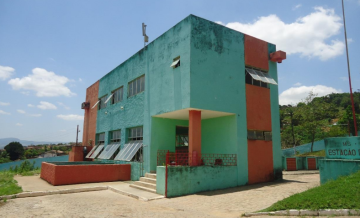
\includegraphics{figures/ETACatende360.png}
%\centerline{\epsffile{ETACatende.eps}}
\end{figure*}

\begin{figure*}[t]%4
\caption{Conventional (left) and mechanical (right) treatment plants.}
\label{fig:WTPConvMec}
\centering
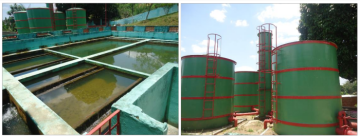
\includegraphics{figures/ETAConvMec360.png}
\end{figure*}

After the adduction, the water captured at the Santa Rita weir, goes to the treatment phases, being received at the WTP through channels, and passing through a flow meter called Calha Pashall. In this trough aluminum sulphate and chlorine are added (Figure \ref{fig:WTPParshall}). These two chemicals help in the coagulation step by reacting with particles that are suspended in raw water. At this stage, the water goes through shares called flocculators, where the added reagents transform the impurities into larger particles to be removed during decantation. 

\begin{figure*}[t]%4
\caption{Parshall gutter, addition of chlorine and aluminum sulphate.}
\label{fig:WTPParshall}
\centering
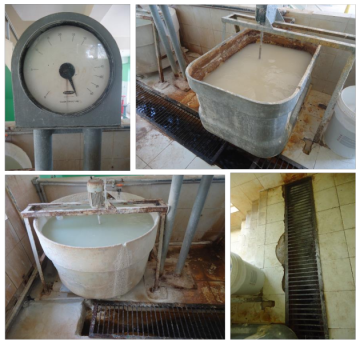
\includegraphics{figures/calhaPashall360.png}
\end{figure*}

The water, then flocculated, goes to another phase, passing through larger layers called decanters, where the flakes formed are deposited in tubular modules similar to a beehive, making the water almost suitable for consumption. In these stages of treatment, almost all contamination factors are eliminated, filtration is then carried out to further improve the decanted water which, by gravity, passes through filters made of a porous medium with the ability to retain and remove impurities even existing in the water. In disinfection, physical or chemical agents are used, such as chlorine, used for the destruction of pathogenic organisms that cause diseases, ending with the correction of pH, where products are also added so that the treated water has a suitable pH for consumption. After being treated, the water is deposited in a supported type reservoir with a capacity of 500,000 m$^3$ of storage (Central Reservoir). Treatment is carried out in continuous flow. 

The water collected from the Bálsamo das Freiras Reservoir is treated in mechanical filters, where the addition of chemical products is carried out automatically. The disposal of the water treated in these filters is also carried out in the Central Reservoir. 

\subsection{Water distribution in Catende}

For the planning of water distribution, the city of Catende was divided into 6 zones (Figure \ref{fig:SectorsCatende}). 

\begin{figure*}[t]%9
\caption{Catende map by supply zones. Source: Adapted from the Archives of the Municipality of Catende, consulted in 2016}
\label{fig:SectorsCatende}
\centering
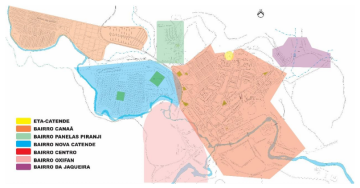
\includegraphics{figures/setores360.png}
\end{figure*}
 
In order to allow water resources to reach consumer units in the most distant neighborhoods from the WTP, capacity studies were carried out, considering the population increase. Based on these studies, the distribution managers identified the need to install reservoirs that serve as water redistribution points. 

The water treated at the WTP - Catende is deposited in a central elevated reservoir (named Central Reservoir), which has a capacity of 500,000 m$^3$ . From this reservoir, it is distributed to another elevated type reservoir with a capacity of 400,000 m$^3$, both located in the WTP. The Elevated Reservoir is responsible for distributing water to the Nova Catende and Jaqueira districts. This reservoir receives water from the
Central Reservoir through pumping, but distributes to the aforementioned neighborhoods through gravitational force. 

\begin{figure*}[t]%4
\caption{Reservoirs raised (left) and elevated (right).} 
\label{fig:reservoiresCatende}
\centering
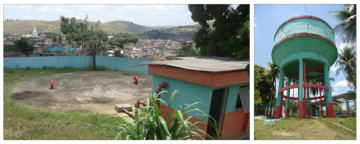
\includegraphics{figures/reservoires360.png}
\end{figure*}

The Central Reservoir, in addition to supplying water to the Elevated Reservoir (in the WTP), also supplies three more reservoirs of the elevated type in the Panelas Piranji, Canaã and Oxifan neighborhoods, with storage capacities of 100,000 m$^3$, 180,000 m$^3$ and 20,000 m$^3$, respectively. The first two mentioned are supplied with the help of two pairs of pumps while the third reservoir is also supplied by gravitational force. The city center, on the other hand, receives water from the central reservoir through gravitational force, as it is directly linked to the WTP. 

Figure \ref{fig:WDSCatende} shows a representation of the water supply network described above. The supplier managers regulates the water supply in Catende, by opening or closing the valves that control the distribution flow. Currently, the company leaves these valves permanently open, maintaining a continuous flow of this resource, with the supply being interrupted only to maintain the treatment filters or the distribution network. 

\begin{figure*}[t]%4
\caption{Water Distribution Scheme in Catende.}
\label{fig:WDSCatende}
\centering
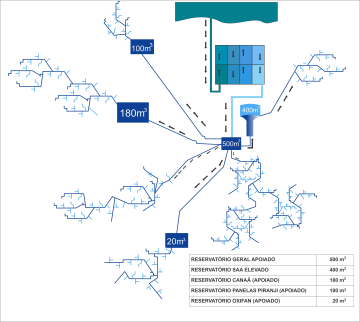
\includegraphics{figures/esquema360.png}
\end{figure*}
 
\subsection{Demand from consumer units}

Based on data obtained from the UN (United Nations), \cite{Paganine2013} informs that 110 liters of water per day are enough to meet a person's basic needs. However, in interviews conducted with WTP administrators in Catende, it was informed that the average consumption per inhabitant in the city was around 200 liters per day. Considering the average consumption reported and data from \cite{IBGECatende} obtained from the 2010 Census, it was estimated that an average of 7,473,960.00 liters of water per day is needed to serve the population of Catende. 

Through the visits carried out at the WTP in Catende in 2016, it was also possible to obtain information on the daily production capacity and the number of households served, separated by the supply zones. Table \ref{tab:SectorsCatende} shows the water demand for each zone (neighborhood), where the necessary amount of water per household was defined considering that each household resides on average 3.9 inhabitants (average established by \cite{IBGECatende} through the last large demographic census of 2010). Information on the number of households/zones and the average water consumption per inhabitant were provided by the WTP managers, considering the average use of 200 liters of water per inhabitant. It was also informed that almost 100\% of households have reservoirs ranging between 500 and 1000 liters. These are activated when water is not supplied, either due to maintenance in the distribution network, or in periods when the water flow for treatment is low, thus limiting the daily supply. 

\begin{table}[t]
\begin{center}
	\begin{tabular}{ c  r  r } 
		supply sector       &  \multicolumn{1}{c}{number of}     &   \multicolumn{1}{c}{average consumption}  \\
		                    &  \multicolumn{1}{c}{households}    &  \multicolumn{1}{c}{(liters/day)}   \\
		\\
		Centro              & 5431          &  4.236.180,00  \\
		Nova Catende        & 1043 			&    813.540,00  \\
		Jaqueira            &  976          &    761.280,00 \\
		Panelas Piranji     &  459          &    358.020,00 \\
		Canaã               & 1538          &  1.199.640,00 \\
		Oxifan              &  135          &    105.300,00 \\
		\\
		Total               & 9582          &  7.473.960,00 \\
		\hline
	\end{tabular}
\caption{Demand by sector - Catende (data from 2016)}
\label{tab:SectorsCatende}
\end{center}
\end{table}

Although Catende is located in a region that does not suffer so much from the lack of water, it has been observed over the years, a considerable drop in its water sources, alerting the population and managers about the need to save this resource. The production capacity of treated water, when the abstraction in water sources is at its maximum limit, is 288,000 liters of water per hour, in this way, in 24 hours it is possible to fill 13.8 reservoirs of 500,000 m$^3$. Observing the total daily demand required, it is concluded that the productive capacity does not meet the daily needs of the population, which highlights the need for good management of water distribution.

Based on this issue, the water distribution problem was then defined, as discussed in the next section. 

\section{Problem of Elaborating Water Distribution Schedules in Periods of Scarcity} 
\label{sec:EWDSPSP}

This water distribution problem arises in times of scarcity, in which it becomes necessary to draw up a distribution schedule for the different zones of the city, based on the limitation of this precious resource. Such schedule informs the shifts in which the inhabitants will be able to acquire treated water, generating their reserves for the periods in which there will be no supply. The following section presents a mathematical modeling for the problem considered in this work. 

\subsection{Mathematical modeling}
\label{sec:problemModel}
 
The symbols used in the model are shown in the Table (\ref{tab:symbols}). And the mathematical model is presented as follows:

\begin{eqnarray}
\label{eq:objFunc}
	maximize \quad V_\mathrm{dist} - \mathrm{FRF} * \sum_{d=1}^{\mathrm{ND}}{\sum_{s=1}^{\mathrm{NS}}{\sum_{z=\mathrm{NR}+1}^{\mathrm{NL}}{|\mathrm{P_{dem}}_{z} - P_{\mathrm{dist}dsz}|}}} \\ \nonumber 
	+ \mathrm{VRF} * \sum_{d=1}^{\mathrm{ND}}{\sum_{s=1}^{\mathrm{NS}}{\sum_{l=1}^{\mathrm{NL}}{X_{dsl}}}} - \mathrm{ICIrF}*C_{\mathrm{idleEWSum}}
\end{eqnarray}

\emph{subj. to}

\begin{equation}
	InF_{dsl} - V_{l} * X_{dsl} = 0, \quad \forall{d, s, l}
	\label{eq:evalInF}
\end{equation}

\begin{equation}
	V_l - {InFR}_l * \mathrm{T} = 0, \quad \forall{l}
	\label{eq:evalnFR}
\end{equation}

\begin{equation}
	{InFR}_l - \mathrm{MaxInfR}_{l} \leq 0, \quad \forall{l}
	\label{eq:evalMaxInfR}
\end{equation} 

\begin{equation}
	{InFR}_l - \mathrm{MinInfR}_{l} \leq 0, \quad \forall{l}
	\label{eq:evalMinInfR}
\end{equation}

The objective function (\ref{eq:objFunc}) at the same time: a) maximizes the volume distributed to the zones (first term); b) makes the distribution of water between the different zones as fair as possible (second term); and c) minimizes the idle capacity of the reservoirs (fourth term). The third term is used to force the uniqueness of the solution (or at least reduce the number of possible solutions). Using the + sign before the term makes the valves remain open as long as possible. The parameters $\mathrm{FRF}$ and $\mathrm{VRF}$ are used to regulate the order of importance of the second and third terms, respectively. And $\mathrm{ICIrF}$ is used to ensure that the algorithm prioritizes meeting demand and that the remaining volume in the reservoirs becomes a secondary concern. The equations in (\ref{eq:evalInF}) and (\ref{eq:evalnFR}) are used to, respectively, determine the water inflow and ideal inflow rate based on the evaluated solution.

\begin{table}[h]
\begin{center}
	\begin{tabular}{ l l } 
		\multicolumn{2}{l}{\emph{indexes}} \\ \\

		$d$ & used to designate a day, $d = 1, ..., \mathrm{ND}$ \\
		$s$ & used to designate a shift of a day, $s = 1, ..., \mathrm{NS}$ \\
		$l$ & used to designate a locations that are part of the water supply system (either zones, reservoirs or WTPs), \\
		& $l  = 1, ..., \mathrm{NL}$\\ \\

		\multicolumn{2}{l}{\emph{parameters}} \\ \\
		$\mathrm{ND}$ & number of days \\
		$\mathrm{NS}$ & number of daily distribution shifts \\
		$\mathrm{NL}$ & number of locations \\ 
		$\mathrm{T}$ & time per shift \\
		$\mathrm{MaxInFR}_{l}$ & maximum inflow rate of the pipeline that reaches the reservoir at the location $l$ \\
		$\mathrm{MinInFR}_{l}$ & minimum inflow rate set for the pipeline that reaches the reservoir at the location $l$ \\
		$\mathrm{FRF}$ & used as relevance factor for the fair distribution \\
		$\mathrm{VRF}$ & used as relevance factor for the adjustment of the valves \\
		 $\mathrm{ICIrF}$ &  irrelevance factor for idle capacity \\ \\

		\multicolumn{2}{l}{\emph{decision variables}} \\ \\

		$X_{dsl} $ & binary variable that receives value 1 when the inlet valve\footnote[1*]{} of location $l$ is open on \\
		& the $s$-th shift of day $d$, and receives value 0 when it is closed in the same period \\
		$V_l$ & ideal volume of water distributed to the location $l$ in any shift in which \\
		& the corresponding valve remains open \\\\ 

		\multicolumn{2}{l}{\emph{secondary variables}} \\ \\

		$InF_{dsl}$ & water inflow received by location $l$ on the $s$-th shift of day $d$ \\
		${InFR}_l$ & ideal inflow rate of location $l$ \\ \\

	\end{tabular}
\caption{Table of symbols used in the mathematical model. 1* Notice that in some cases the valves are replaced by pumps. In these cases, the pumps can be compared to open valves, when activated, and closed valves, when not activated. Therefore, the simplification adopted (considering only valves) does not generate any implications for the developed model.}
\label{tab:symbols}
\end{center}
\end{table}
\subsubsection{Decision variables}

As informed in this work, the municipality carries out the distribution planning for the various zones and reservoirs considering distribution shifts. On each shift, water release is controlled by opening or closing valves. Thus, in each considered shift, there are two possible states for each valve - open (when it allows the transfer of water from one point to another) and closed (when it does not allow this transfer of water). Therefore, the water distribution problem basically consists of defining for each valve and for each shift, whether the valve will be open or closed, so that the primary decision variables considered in the model can be defined by the binary variables $X_{dsl} $, where:
 

\subsubsection{Objective function}




The  In this work we adopt $\mathrm{IrF_{idleness}} = 0.000005$. 

The other parameters, variables and terms of the objective function are detailed in the restrictions section presented below. 



Based on the equations and inequalities presented in (\ref{evalVolIn}) to (\ref{eq:resEvalInFRMin}) we can then determine the daily outflow of each location $l$ in each shift $s$, $V_{\mathrm{out}dsl}$.

For the case of reservoirs, the volume of water supplied by the reservoir $r$ at the end of the $s$-th shift of the day $d$, $V_{\mathrm{out}dsr}$, can be defined by:

\begin{eqnarray} 
    \label{eq:evalVoutRes}
	\mathrm{V_{out}}_{dsr} = \sum_{l=1}^{\mathrm{NL}}{(V_{\mathrm{in}dsl}*\mathrm{Y}_{rl})}, \\ 
	\quad d = 1, ..., \mathrm{ND}, \quad s = 1, ..., \mathrm{NS}, \quad r=1, ..., \mathrm{NR} \nonumber
\end{eqnarray}

\noindent where the binary variable $\mathrm{Y}_{rl}$ informs the physical structure of the water distribution system:

\begin{eqnarray}
    \label{eqFisDist}
	\mathrm{Y}_{rl} = 
	\begin{cases}
		1  & \text{if water is supplied directly from the reservoir } r \text{ to the location } l \\ 
		0  & \text{if water is not supplied directly from the reservoir  } r \text{ to the location } l \\
	\end{cases} \\ \nonumber
	r = 1, ..., \mathrm{NR}, \quad l = 1, ..., \mathrm{NL} \nonumber
\end{eqnarray}

Furthermore, the inflows and outflows in the network are related through the flow equations in (\ref{eqVolRemT1}) and (\ref{eqVolRem!T1}):

\begin{eqnarray}
    \label{eqVolRemT1}
	V_{\mathrm{rem}dsl} = V_{\mathrm{rem}(d-1)(\mathrm{NS})l} + V_{\mathrm{in}dsl} - V_{\mathrm{out}dsl}, \\ 
	\quad d = 1, ..., \mathrm{ND}, \quad s = 1, \quad l=1, ..., \mathrm{NL} \nonumber
\end{eqnarray}

\noindent and

\begin{eqnarray}
    \label{eqVolRem!T1}
	V_{\mathrm{rem}dsl} = V_{\mathrm{rem}d(s-1)l} + V_{\mathrm{in}dsl} - V_{\mathrm{out}dsl}, \\ 
	\quad d = 1, ..., \mathrm{ND}, \quad s= 2, ..., \mathrm{NS}, \quad l=1, ..., \mathrm{NL} \nonumber
\end{eqnarray}

\noindent where $V_{\mathrm{rem}dsl}$ represents the volume of water remaining in the reservoir at location $l$ at the end of the $s$-th shift of the day $d$, being $V_{\mathrm{rem}0(\mathrm{NS})l}$ a constant defined by the initial reservoir volume at location $l$, $\mathrm{V_{ini}}_l$:
 
\begin{equation}
	V_{\mathrm{rem}dsl} = \mathrm{V_{ini}}_l, \quad d = 0, \quad s = \mathrm{NS}, \quad l=1, ..., \mathrm{NL}
	\label{EqVolRemD0}
\end{equation}

It is also necessary to consider that the remaining volumes in the reservoirs must not be negative and must always be less than their respective capacities, $\mathrm{C}_{l}$.

\begin{equation}
	V_{\mathrm{rem}dsl} \geq 0, \quad d = 1, ..., \mathrm{ND}, \quad s = 1, ..., \mathrm{NS}, \quad l=1, ..., \mathrm{NL}
\end{equation}

\noindent and

\begin{equation}
	V_{\mathrm{rem}dsl} \leq \mathrm{C}_{l}, \quad d = 1, ..., \mathrm{ND}, \quad s = 1, ..., \mathrm{NS}, \quad l=1, ..., \mathrm{NL}
\end{equation}

In the case of the zones, the total daily volume distributed to each zone will be limited by the daily demand of that zone, $\mathrm{D}_z$:

\begin{equation}
	\sum_{s=1}^{\mathrm{NS}}{V_{\mathrm{out}dsz}} \leq \mathrm{D}_z, \quad d = 1, ..., \mathrm{ND}, \quad z=\mathrm{NR}+1, ..., \mathrm{NL}
	\label{ResDemand}
\end{equation}

The total amount of water distributed by the zones, $V_\mathrm{dist}$, is then defined by the sum:

\begin{equation}
V_\mathrm{dist} = \sum_{z=\mathrm{NR}+1}^{\mathrm{NL}}{V_{\mathrm{out}z}}
\end{equation}

\noindent where $V_{\mathrm{out}z}$ represents the total outflow of zone $z$:

\begin{equation}
V_{\mathrm{out}z} = \sum_{d=1}^{\mathrm{ND}}\sum_{s=1}^{\mathrm{NS}}{V_{\mathrm{out}dsz} }, \quad z=\mathrm{NR}+1, ..., \mathrm{NL}
\label{evalVolInZone}
\end{equation}

\noindent and $V_{\mathrm{out}dsz}$ represents the outflow of zone $z$ at the end of the $s$-th shift of the day $d$. 

Regarding the second term of the objective function, we consider in this work that, in a fair distribution, the volume proportions distributed in each shift by each zone $z$ are as close as possible to its demand proportion, $\mathrm{P_ {dem}}_{z}$:

\begin{equation}
	\mathrm{P_{dem}}_{z} = \mathrm{D_{shift}}_z / \mathrm{D_{total}}
\end{equation}

\noindent being $\mathrm{D_{total}}$ the total demand:

\begin{equation}
	\mathrm{D_{total}} = \sum_{z=\mathrm{NR}+1}^{\mathrm{NL}}{\mathrm{D}_z}
\end{equation}

\noindent and $\mathrm{D_{shift}}_z$ the demand per shift of zone $z$:

\begin{equation}
	\mathrm{D_{shift}}_z = \mathrm{D}_z / (\mathrm{ND} * \mathrm{NS}), \quad z=\mathrm{NR}+1, ..., \mathrm{NL}
	\label{evalDemandByShift}
\end{equation}

\noindent where the daily demand of zone $z$, $\mathrm{D}_z$, is defined by:

\begin{equation}
	\mathrm{D}_z = \mathrm{C_{average}} * \mathrm{HC} * \mathrm{NH}_z, \quad z=\mathrm{NR}+1, ..., \mathrm{NL}
\end{equation}

\noindent such that $\mathrm{C_{average}}$ represents the average daily consumption per inhabitant, $\mathrm{HC}$ represents the housing coefficient, and $\mathrm{NH}_z$ the number of households in the zone $z$.

The proportions of volume distributed in each shift by each zone, $P_{\mathrm{dist}dsz}$, are defined by:

\begin{equation}
	P_{\mathrm{dist}dsz} = V_{\mathrm{out}dsz} / V_\mathrm{dist} , \quad z=\mathrm{NR}+1, ..., \mathrm{NL}
\end{equation}


The third term of the objective function seeks to ensure that the flow is distributed among the shifts, except when this distribution is bounded by flow restrictions. 

Finally, the fourth term deals with another important issue to be considered: the idle capacity of the reservoirs. At the end of the last shift of each day, it is desired that the remaining reservoir volumes, $V_{\mathrm{rest}dsl}$, are as close to their respective capacities, $\mathrm{C}_l$, as possible.

Once the remaining volumes in the reservoirs have been defined, it is then possible to determine the idle capacities of the latter in each shift, $C_{\mathrm{idle}dsl}$, through the Eqs. in (\ref{EqIdleCap}):

\begin{equation}
	C_{\mathrm{idle}dsl} = \mathrm{C}_{l} - V_{\mathrm{rem}dsl}, \quad d = 1, ..., \mathrm{ND}, \quad \quad s = 1, ..., \mathrm{NS}, \quad l=1, ..., \mathrm{NL}
	\label{EqIdleCap}
\end{equation}

\noindent being the exponentially weighted sum of idle capacities, computed in the last shifts of each day, $C_{\mathrm{idleEWSum}}$, defined by:

\begin{equation}
	C_{\mathrm{idleEWSum}} = \sum_{d=1}^{\mathrm{ND}}{\sum_{l=1}^{\mathrm{NL}}{  (C_{\mathrm{idle}ds({\mathrm{NS}})})^{\mathrm{RF}_l }    }}
	\label{EqIdleCapEWSum}
\end{equation}

\noindent where $\mathrm{RF}_l$ represents the importance attributed to maintaining water in each reservoir, since there is a surplus of water to fill the reservoirs. It is important that the values of these parameters are greater than and close to 1.00. In this work, we adopted: $1.13$ for the WTP ($r=1$) and for the Central Reservoir ($r=2$); 1.12 for the other reservoirs; and $1.00$ for the zones.

Note that, in the case of zones, each zone $z$ is considered to have a single reservoir, whose capacity is defined by the sum of the capacities of the various housing reservoirs in the zone.

\begin{equation}
	\mathrm{C}_z =  \mathrm{C_{averReserv}}_z * \mathrm{NH}_z, \quad z=\mathrm{NR}+1, ..., \mathrm{NL}
\end{equation}

\noindent where $\mathrm{C_{averReserv}}_z$ represents the average of the reservoir capacities of the households in the zone $z$.

\subsubsection{Distribution time adjustment}

In order to guarantee a fair distribution, in specific cases where the actual flows are greater than the ideal flows informed in the initial model solution, and cannot be reduced in practice, it is necessary to limit the water distribution time for certain locations. In this case, the proper distribution time per shift for local $l$, $T_{\mathrm{adeq}l}$, can be defined according to equations in (\ref{eq:evalTimeAdq}). In practice, once delivery times are adequately limited, water delivery will proceed as planned.

\begin{equation}
	T_{\mathrm{adeq}l} = \mathrm{T} * ({FR}_l / \mathrm{FR_{max}}_{l}), \quad l=1, ..., \mathrm{NL}
	\label{eq:evalTimeAdq}
\end{equation}

\subsection{Tests and results}

To validate the proposed model, a LINGO code was developed and ran in the 'global solver' mode, using the parameter values recommended by the software \cite{LINGO}. The tests were carried out based on the considerations presented in the sections \ref{sec:initialConsiderations}, \ref{sec:praticalAspects} and \ref{sec:limitations} and using the data collected during this work, as summarized in the section \ref{sec:data}. The results found as well as an analysis of these results are presented along the following sections together with the considerations studied. 

\subsubsection{Data collected}
\label{sec:data}

Tables \ref{tab:weirsCatende}, \ref{tab:reservoirsCatende}, \ref{tab:zonesCatende} and \ref{tab:phyDitStr} present a synthesis of the data referring to the weirs, reservoirs, zones and the network of studied water distribution, respectively. The conceptual and mathematical model presented in this paper, as well as the solver used to validate the model, were developed through a recent effort. However, the data presented in this section were collected in 2016 as part of an extension project carried out by the authors of this article, through which a detailed study of the water distribution process presented in the section \ref{sec:CatendeWDS} was carried out \citep{CandidoEtAl2016}. 

\noindent number of locations (NL) = 12 (6 zones) 

\noindent number of reservoirs (NR) = 6 (1 WTP) 

\noindent housing coefficient ($\mathrm{HC}$) = 3.9 inhabitants / household 

\noindent average daily inflow per inhabitant ($\mathrm{C_{average}}$) = 200 liters / inhabitant * day 

\noindent Note: each weir supplies water to an WTP (conventional or mechanical). However, both supply water to the Central Reservoir. For this reason, in this work we consider only a single WTP. 

\begin{table}[t]
\begin{center}
	\begin{tabular}{ c  c  c } 
		weir      & name        & distribution flow rate  ($\mathrm{liters/hour}$)     \\
		                                                                    \\
		1              & Santa Rita weir            & 241.200,00          \\
		2              & Bálsamo das Freiras  weir  & 126.000,00         \\
							                                                \\
		\hline
		Total          &                               & 367.200,00         \\
		\\
	\end{tabular}
\caption{Weirs data - Catende (data from 2016)}
\label{tab:weirsCatende}
\end{center}
\end{table}

\begin{table}[t]
\begin{center}
	\begin{tabular}{ c  c  c  c } 
		reservoir      & name              & capacity                       & Maximum inflow rate informed    \\
		($r$)          &             	   &  ($\mathrm{C}_{r}$) (m$^3$)    &  ($\mathrm{InFR_{max}}_{r}$) ($\mathrm{liters/hour}$) \\
		\\
		1              & WTP               & 2.500.000            &  367.200,00   \\
		2              & Central           &   500.000 			  &  288.000,00   \\
		3              & Elevated          &   400.000            & não informado \\
		4              & Panelas Piranji   &   100.000            & não informado \\
		5              & Canaã             &   180.000            & não informado \\
		6              & Oxifan            &    20.000            & não informado \\
		\\
	\end{tabular}
\caption{Reservoirs data - Catende (data from 2016)}
\label{tab:reservoirsCatende}
\end{center}
\end{table}

\begin{table}[t]
\begin{center}
	\begin{tabular}{ c  c  c } 
		zone          & name         & Number of households \\
		($z$)          &              & ($\mathrm{NH}_{z}$)   \\
		                                               \\
		7              & Centro           & 5.431 \\
		8              & Nova Catende     & 1.043 \\
		9              & Jaqueira         &   976 \\
	   10              & Panelas Piranji  &   459 \\
	   11              & Canaã            & 1.538 \\
	   12              & Oxifan           &   135 \\
	   \\
	\end{tabular}
\caption{Zones data - Catende (data from 2016)}
\label{tab:zonesCatende}
\end{center}
\end{table}

\begin{table}[t]
\begin{center}
	\begin{tabular}{ c c c c c c c c c c c c c } 

		($\mathrm{Y}_{rl}$)	& 1 & 2 & 3 & 4 & 5 & 6 & 7 & 8 & 9 & 10 & 11 & 12  \\
		                                                                      \\
		1	              	& 0 & 1 & 0 & 0 & 0 & 0 & 0 & 0 & 0 &  0 &  0 &  0  \\
		2                 	& 0 & 0 & 1 & 1 & 1 & 1 & 1 & 0 & 0 &  0 &  0 &  0  \\
		3                 	& 0 & 0 & 0 & 0 & 0 & 0 & 0 & 1 & 1 &  0 &  0 &  0  \\
		4                 	& 0 & 0 & 0 & 0 & 0 & 0 & 0 & 0 & 0 &  1 &  0 &  0  \\
		5                 	& 0 & 0 & 0 & 0 & 0 & 0 & 0 & 0 & 0 &  0 &  1 &  0  \\
	    6                 	& 0 & 0 & 0 & 0 & 0 & 0 & 0 & 0 & 0 &  0 &  0 &  1  \\
	\end{tabular}
\caption{Physical distribution structure - Catende (data from 2016)}
\label{tab:phyDitStr}
\end{center}
\end{table}

\subsubsection{Initial considerations}
\label{sec:initialConsiderations}

Figure \ref{fig:evalOptimalValues} presents the optimal solution for the data summarized in the section \ref{sec:data}, calculated with the aid of the 'LibreOffice Calc' software, considering the maximum daily distribution value (in a 24-hour shift), limited by the outflows of the weirs and the WTP (case 01). 

\begin{figure*}[t]
	\begin{center}
	    \caption{Determination of optimal distribution values with 'LibreOffice Calc', considering a daily 24-hour distribution period}
		\label{fig:evalOptimalValues}
		\centering
		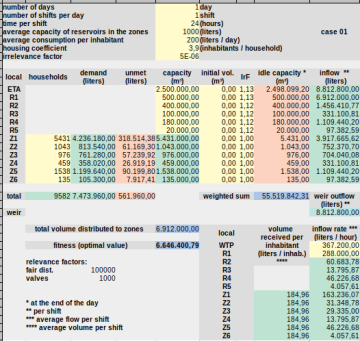
\includegraphics{figures/fit360.png}
	\end{center}
\end{figure*}

As we can see in this figure, the optimal daily water distribution volume per inhabitant, considering a daily 24-hour distribution period, is 184.96 liters / (day * inhabitant). Therefore, we can conclude that, in fact, the flow of the pipeline that transports water from the WTP ($r=1$) to the Central Reservoir ($r=2$) is not sufficient to meet the average daily consumption of the population informed by the company (200 liters / (day * inhabitant)).

Another important piece of information that we observe in this figure are the ideal inflow rates, which would result in a fair distribution for the population of Catende. These values are basically defined as a function of water availability, demands, and initial volumes in the reservoirs. Such values were identified using the following calculation logic:

\noindent 1) as the part of the inflow received by the WTP and not distributed is completely used to fill its reservoir and, as the inflow rate of the Central Reservoir is lower than the inflow rate of the WTP, so $V_{\mathrm{in}dsr}$, for the WTP and the Central Reservoir, are calculated according to Eqs. in \ref{eq:volInFRCentral}: 

\begin{equation}
	V_{\mathrm{in}dsr} = \mathrm{InFR_{max}}_r * \mathrm{T}, \quad d = 1, \quad s = 1, \quad r = 1,2
	\label{eq:volInFRCentral}
\end{equation}

\noindent 2) the total availability of water, released by the Central Reservoir, which directly or indirectly supplies all other reservoirs and zones, is less than the total demand. Therefore, the volume of water received by the Central Reservoir is completely distributed to the zones (and not to fill the reservoirs), with the fair distribution being proportional to the number of households in each zone: 

\begin{eqnarray}
	V_{\mathrm{in}dsz} = V_{\mathrm{in}dsr} * (\mathrm{ND}_z / \mathrm{ND_{total}}), \\
	\quad d = 1, \quad s = 1, \quad r = 2, \quad z=\mathrm{NR}+1, ..., \mathrm{NL} \nonumber
\end{eqnarray}

\noindent and, 3) as the volumes received by the reservoirs are completely distributed: 

\begin{equation}
	\mathrm{V_{in}}_{dsr} = \mathrm{V_{out}}_{dsr} \quad d = 1, \quad s = 1, \quad r=3, ..., \mathrm{NR}
\end{equation}

\noindent being the values of $V_{\mathrm{out}dsr}$ calculated according to the Eqs. in (\ref{eq:evalVoutRes}) recursively, and the ideal rates (not informed) then calculated based on the Eqs. in (\ref{eqEvalFR}).

After performing the calculations shown in Figure \ref{fig:evalOptimalValues}, we run the solver in Lingo, using the same inputs shown in this figure, along with other data reported in the \ref{sec:data} section. The values 367,200.00 and 288,000.00 were used as the values of the maximum inflow rates informed for the WTP ($r=1$) and for the Central Reservoir ($r=2$), respectively. No limit values for inflow rates were informed for the other reservoirs and zones. Table \ref{tab:lingoEvalCase01} displays the values found by the solver. As we can see in this table, the solver found the calculated optimal values very quickly and with a very small margin of error. 

\begin{table}[t]
\begin{center}
\begin{small}
	\begin{tabular}{ c r r r r r } 
		location & \multicolumn{1}{c}{total demand}      & \multicolumn{1}{c}{capacity} & \multicolumn{1}{c}{initial vol.} & \multicolumn{1}{c}{idle capacity **} & \multicolumn{1}{c}{total inflow}  \\
		      & \multicolumn{1}{c}{(liters)} & \multicolumn{1}{c}{(m$^3$)}   & \multicolumn{1}{c}{(m$^3$)}     &  \multicolumn{1}{c}{(m$^3$)}   &  \multicolumn{1}{c}{(liters)}               \\
		\\
		WTP   &              & 2,500,000.00 & 0.00 &  2498,099.20 & 8,812,800.00 \\
		R1    &              &   500,000.00 & 0.00 &    500,000.00 & 6,912,000.00 \\
		R2    &              &   400,000.00 & 0.00 &    400,000.00 & 1,456,410.77 \\
		R3    &              &   100,000.00 & 0.00 &    100,000.00 &   331,100.81 \\
	    R4    &              &   180,000.00 & 0.00 &    180,000.00 & 11,094,40.20 \\
	    R5    &              &    20,000.00 & 0.00 &     20,000.00 &    97,382.59 \\
	    Z1    & 4,236,180.00 & 5,431,000.00 & 0.00 &  5,431,000.00 & 3,917,665.62 \\
	    Z2    &   813,540.00 & 1,043,000.00 & 0.00 &  1,043,000.00 &   752,370.69 \\
	    Z3    &   761,280.00 &   976,000.00 & 0.00 &    976,000.00 &   704,040.07 \\
	    Z4    &   358,020.00 &   459,000.00 & 0.00 &    459,000.00 &   331,100.81 \\
	    Z5    & 1,199,640.00 & 1,538,000.00 & 0.00 &  1,538,000.00 & 1,109,440.20 \\
	    Z6    &   105,300.00 &   135,000.00 & 0.00 &    135,000.00 &    97,382.59 \\
	    \\
	    total & 7,473,960.00 & \multicolumn{2}{r}{exp. weighted sum:} & 55,519,842.31 &              \\
		   \\
		&  &      &  \multicolumn{1}{c}{location}    & \multicolumn{1}{c}{valve status} & \multicolumn{1}{c}{ideal inflow rate}   \\
		\multicolumn{2}{c}{shift data}     &   &      & \multicolumn{1}{c}{} & \multicolumn{1}{c}{(liters/hour)} \\
		   \\
		1   &  \multicolumn{1}{l}{day}   &              		& \multicolumn{1}{c}{WTP}    & \multicolumn{1}{c}{open} &  367,200.00* \\
		1   &  \multicolumn{1}{l}{shif}  &         			    & \multicolumn{1}{c}{R1}     & \multicolumn{1}{c}{open} &  288,000.00* \\
		24  &  \multicolumn{1}{l}{hours/shift}        &         & \multicolumn{1}{c}{R2}     & \multicolumn{1}{c}{open} &    60,683.78 \\
	   &      &              									& \multicolumn{1}{c}{R3}     & \multicolumn{1}{c}{open} &    13,795.87 \\
	   \multicolumn{3}{c}{total zones outflow}                  & \multicolumn{1}{c}{R4}     & \multicolumn{1}{c}{open} &    46,226.68 \\
	   \multicolumn{3}{c}{(liter/shift)}              			& \multicolumn{1}{c}{R5}     & \multicolumn{1}{c}{open} &     4,057.61 \\
	   &      &              									& \multicolumn{1}{c}{Z1}     & \multicolumn{1}{c}{open} &   163,236.07 \\
	   \multicolumn{3}{c}{6,912,000.02}              			& \multicolumn{1}{c}{Z2}     & \multicolumn{1}{c}{open} &    31,348.78 \\
	      &              &              						& \multicolumn{1}{c}{Z3}     & \multicolumn{1}{c}{open} &    29,335.00 \\
	   \multicolumn{3}{c}{optimal value (fitness)}              & \multicolumn{1}{c}{Z4}     & \multicolumn{1}{c}{open} &    13,795.86 \\
	   &             &             						 		& \multicolumn{1}{c}{Z5}     & \multicolumn{1}{c}{open} &    46,226.67 \\
	   \multicolumn{3}{c}{6,646,400.78}              			& \multicolumn{1}{c}{Z6}     & \multicolumn{1}{c}{open} &     4,057.61 \\
	   \\
	   \multicolumn{3}{c}{(computational time  = 4.62 sec)}     & \multicolumn{3}{c}{* values reported for maximum inflow rates} \\
	   \multicolumn{3}{c}{(total number of iterations = 2848)}   & \multicolumn{3}{c}{** at the end of the evaluated period} 
	\end{tabular}
		\end{small}
\caption{Summary of results generated by the solver developed in Lingo for case 01}
\label{tab:lingoEvalCase01}
\end{center}
\end{table}

Very close values were found for fitness and volumes distribution when the solver in Lingo was run considering 3 shifts of 8h (case 03). In this case, the inflow is distributed between the shifts, keeping the same ideal inflow rates. The computational effort increased considerably: computational time = 9.82 sec; and total number of iterations = 5,709.

\begin{table}[t]
\begin{center}
\begin{small}
	\begin{tabular}{ c r r r r r } 
		location & \multicolumn{1}{c}{total demand}      & \multicolumn{1}{c}{capacity} & \multicolumn{1}{c}{initial vol.} & \multicolumn{1}{c}{idle capacity **} & \multicolumn{1}{c}{total inflow}  \\
		      & \multicolumn{1}{c}{(liters)} & \multicolumn{1}{c}{(m$^3$)}   & \multicolumn{1}{c}{(m$^3$)}     &  \multicolumn{1}{c}{(m$^3$)}   &  \multicolumn{1}{c}{(liters)}               \\
		\\
		WTP   &              & 2,500,000.00 & 0.00 &  2,498,099.20 & 8,812,800.00 \\
		R1    &              &   500,000.00 & 0.00 &    500,000.00 & 6,912,000.00 \\
		R2    &              &   400,000.00 & 0.00 &    400,000.00 & 1,456,411.09 \\
		R3    &              &   100,000.00 & 0.00 &    100,000.00 &   331,100.96 \\
	    R4    &              &   180,000.00 & 0.00 &    180,000.00 & 1,109,438.02 \\
	    R5    &              &    20,000.00 & 0.00 &     20,000.00 &    97,382.57 \\
	    Z1    & 4,236,180.00 & 5,431,000.00 & 0.00 &  5,431,000.00 & 3,917,667.30 \\
	    Z2    &   813,540.00 & 1,043,000.00 & 0.00 &  1,043,000.00 &   752,371.02 \\
	    Z3    &   761,280.00 &   976,000.00 & 0.00 &    976,000.00 &   704,040.07 \\
	    Z4    &   358,020.00 &   459,000.00 & 0.00 &    459,000.00 &   331,100.95 \\
	    Z5    & 1,199,640.00 & 1,538,000.00 & 0.00 &  1,538,000.00 & 1,109,438.02 \\
	    Z6    &   105,300.00 &   135,000.00 & 0.00 &    135,000.00 &    97,382.63 \\
	    \\
	    total & 7,473,960.00 & \multicolumn{2}{r}{exp. weighted sum:} & 55,519,842.31 &              \\
		   \\
		&  &      &  \multicolumn{1}{c}{location}    & \multicolumn{1}{c}{valve status} & \multicolumn{1}{c}{ideal inflow rate}   \\
		\multicolumn{2}{c}{shift data}     &   &      & \multicolumn{1}{c}{T1,T2 and T3} & \multicolumn{1}{c}{(liters/hour)} \\
		   \\
		1   &  \multicolumn{1}{l}{day}   &              	& \multicolumn{1}{c}{WTP} & \multicolumn{1}{c}{open} &  367,200.00* \\
		1   &  \multicolumn{1}{l}{shif}  &         			& \multicolumn{1}{c}{R1}  & \multicolumn{1}{c}{open} &  288,000.00* \\
		24  &  \multicolumn{1}{l}{hours/shift}        &     & \multicolumn{1}{c}{R2}  & \multicolumn{1}{c}{open} &   60,683.78  \\
	   &      &              								& \multicolumn{1}{c}{R3}  & \multicolumn{1}{c}{open} &   13,795.87  \\
	   \multicolumn{3}{c}{total zones outflow}              & \multicolumn{1}{c}{R4}  & \multicolumn{1}{c}{open} &   46,226.68  \\
	   \multicolumn{3}{c}{(liters)}              		    & \multicolumn{1}{c}{R5}  & \multicolumn{1}{c}{open} &    4,057.60  \\
	   &      &              								& \multicolumn{1}{c}{Z1}  & \multicolumn{1}{c}{open} &  163,236.07  \\
	   \multicolumn{3}{c}{6,912,000.00}              		& \multicolumn{1}{c}{Z2}  & \multicolumn{1}{c}{open} &   31,348.77  \\
	      &              &              					& \multicolumn{1}{c}{Z3}  & \multicolumn{1}{c}{open} &   29,335.00  \\
	   \multicolumn{3}{c}{optimal value (fitness)}          & \multicolumn{1}{c}{Z4}  & \multicolumn{1}{c}{open} &   13,795.87  \\
	   &             &             						 	& \multicolumn{1}{c}{Z5}  & \multicolumn{1}{c}{open} &   46,226.68  \\
	   \multicolumn{3}{c}{6,670,400.71}                     & \multicolumn{1}{c}{Z6}  & \multicolumn{1}{c}{open} &    4,057.61 \\
	   \\
	   \multicolumn{3}{c}{(computational time  = 9.82 sec)}     & \multicolumn{3}{c}{* values reported for maximum inflow rates} \\
	   \multicolumn{3}{c}{(total number of iterations = 5,709)}   & \multicolumn{3}{c}{** at the end of the evaluated period} 
	\end{tabular}
		\end{small}
\caption{Summary of results generated by the solver developed in Lingo for case 03}
\label{tab:lingoEvalCase03}
\end{center}
\end{table}

\subsubsection{Practical aspects}
\label{sec:praticalAspects}

It would be ideal if the company could regulate the flow rates for water distribution, adjusting these rates according to each ideal solution found by the solver for the different cases evaluated by the planners. However, in practice this becomes very difficult. The following situations will be faced when looking for solutions to real problems:

\begin{itemize}
\item (1) real flow rates of the pipelines smaller than the calculated ideal flow rates;
\item (2) actual pipelines flow rates greater than the calculated ideal flow rates;
\item and (3) very small ideal flow rates, making the supply unsatisfactory.
\end{itemize}

Situations (1) and (3) can be easily solved by indicating maximum and minimum values, respectively, for the inflow rates calculated by the solver. However, care must be taken not to set values that make the problem unresolvable. The planner must always keep in mind that the water distribution network and the flow rates form a single system, with values that are essentially integrated.

In the case of situation (1), as the solver seeks to maximize the volume of water distributed to the zones, the volume of distribution (limited by the inflow rate) in a given location will be transferred to other locations seeking to meet the demand and, later, distributed to filling the idle capacity of the reservoirs. For example, Table \ref{tab:lingoEvaluationsCase22} presents the results found by the solver for case 22, in which the same data used in case 06 were considered, except that a maximum flow rate was informed for zone $\mathrm{Z1}$ ($z = 7$), $\mathrm{InFR_{max}}_7 = $130,000.00 liters/hour (case 06 is just like case 03 but with 2 days).

\begin{table}[t]
\begin{center}
\begin{small}
	\begin{tabular}{ c r r r r r } 
		location & \multicolumn{1}{c}{total demand}      & \multicolumn{1}{c}{capacity} & \multicolumn{1}{c}{initial vol.} & \multicolumn{1}{c}{idle capacity **} & \multicolumn{1}{c}{total inflow}  \\
		      & \multicolumn{1}{c}{(liters)} & \multicolumn{1}{c}{(m$^3$)}   & \multicolumn{1}{c}{(m$^3$)}     &  \multicolumn{1}{c}{(m$3$)}   &  \multicolumn{1}{c}{(liters)}               \\
		\\
		WTP   &               & 2,500,000.00 & 0.00 &  2,495,089.96 & 17,625,600.00 \\
		R1    &               &   500,000.00 & 0.00 &    500,000.00 & 12,715,560.00 \\
		R2    &               &   400,000.00 & 0.00 &    400,000.00 &  3,149,640.00 \\
		R3    &               &   100,000.00 & 0.00 &    100,000.00 &    716,040.00 \\
	    R4    &               &   180,000.00 & 0.00 &    180,000.00 &  2,399,280.00 \\
	    R5    &               &    20,000.00 & 0.00 &     20,000.00 &    210,600.00 \\
	    Z1    &  8,472,360.00 &     5,431.00 & 0.00 &      5,431.00 &  6,240,000.00 \\
	    Z2    &  1,627,080.00 &     1,043.00 & 0.00 &      1,043.00 &  1,627,080.00 \\
	    Z3    &  1,522,560.00 &       976.00 & 0.00 &        976.00 &  1,522,560.00 \\
	    Z4    &    716,040,00 &       459.00 & 0.00 &        459.00 &    716,040.00 \\
	    Z5    &  2,399,280.00 &     1,538.00 & 0.00 &      1,538.00 &  2,399,280.00 \\
	    Z6    &    210,600.00 &       135.00 & 0.00 &        135.00 &    210,600.00 \\
	    \\
	    total & 14,947,920,00 & \multicolumn{2}{r}{exp. weighted sum:} & 110,966,229.48 & \\
		   \\
		&  &      &  \multicolumn{1}{c}{location}    & \multicolumn{1}{c}{valve status}         & \multicolumn{1}{c}{ideal inflow rate}   \\
		\multicolumn{2}{c}{shift data}     &   &      & \multicolumn{1}{c}{T1 and T2}        & \multicolumn{1}{c}{(liters/hour)}  \\
		   \\
		2   &  \multicolumn{1}{l}{day}   &              		& \multicolumn{1}{c}{WTP}    & \multicolumn{1}{c}{open} &  367,200.00* \\
		3   &  \multicolumn{1}{l}{shift}  &         			& \multicolumn{1}{c}{R1}     & \multicolumn{1}{c}{open} &  264,907.50  \\
		8   &  \multicolumn{1}{l}{hours/shift}        &         & \multicolumn{1}{c}{R2}     & \multicolumn{1}{c}{open} &   65,617.50  \\
	   &      &              									& \multicolumn{1}{c}{R3}     & \multicolumn{1}{c}{open} &   14,917.50  \\
	   \multicolumn{3}{c}{total zones outflow}                  & \multicolumn{1}{c}{R4}     & \multicolumn{1}{c}{open} &   49,985.00  \\
	   \multicolumn{3}{c}{(liters)}              				& \multicolumn{1}{c}{R5}     & \multicolumn{1}{c}{open} &    4,387.50  \\
	   &      &              									& \multicolumn{1}{c}{Z1}     & \multicolumn{1}{c}{open} &  130,000.00* \\
	   \multicolumn{3}{c}{12,715,560.00}              			& \multicolumn{1}{c}{Z2}     & \multicolumn{1}{c}{open} &   33,897.50  \\
	      &              &              						& \multicolumn{1}{c}{Z3}     & \multicolumn{1}{c}{open} &   31,720.00  \\
	   \multicolumn{3}{c}{optimal value (fitness)}              & \multicolumn{1}{c}{Z4}     & \multicolumn{1}{c}{open} &   14,917.50  \\
	   &             &             						 		& \multicolumn{1}{c}{Z5}     & \multicolumn{1}{c}{open} &   49,985.00  \\
	   \multicolumn{3}{c}{12,217,517.79}              			& \multicolumn{1}{c}{Z6}     & \multicolumn{1}{c}{open} &    4,387.50  \\
	   \\
	   \multicolumn{3}{c}{(computational time = 5.01 sec)} & \multicolumn{3}{c}{* values reported for maximum inflow rates} \\
	   \multicolumn{3}{c}{(total number of iterations = 1,030)} & \multicolumn{3}{c}{** at the end of the evaluated period} 

	\end{tabular}
\caption{Summary of results generated by the solver developed in Lingo for case 22}
\label{tab:lingoEvaluationsCase22}
\end{small}
\end{center}
\end{table}

For situation (3), once a minimum value is indicated for the inflow of a given location, the solver will propose solutions in which the inflow of some locations will be null or concentrated in one or a few shifts. For example, Table \ref{tab:lingoEvaluationsCase23} presents the results found by the solver for case 23, in which the same data used in case 06 were considered, except that a minimum flow rate was reported for the reservoir $\mathrm{R5}$ ($r=6$), $\mathrm{InFR_{min}}_6 = $5,000.00 liters/hour. As we can see in this table, the inflow of reservoir $\mathrm{R5}$ and zone $\mathrm{Z6}$ received value 0 for the first shift of the first day. The solver presented a result for case 23 after setting the parameter value $\mathrm{RF_{valves}}=10,000$.

\begin{table}[t]
\begin{center}
\begin{small}
	\begin{tabular}{ c r r r r r } 
		location & \multicolumn{1}{c}{total demand}      & \multicolumn{1}{c}{capacity} & \multicolumn{1}{c}{initial vol.} & \multicolumn{1}{c}{idle capacity **} & \multicolumn{1}{c}{total inflow}  \\
		      & \multicolumn{1}{c}{(liters)} & \multicolumn{1}{c}{(m$^3$)}   & \multicolumn{1}{c}{(m$^3$)}     &  \multicolumn{1}{c}{(m$3$)}   &  \multicolumn{1}{c}{(liters)}               \\
		\\
		WTP   &               & 2,500,000.00 & 0.00 &  2496,198.40 & 17,625,600.00 \\
		R1    &               &   500,000.00 & 0.00 &    500,000.00 & 13,824,000.00 \\
		R2    &               &   400,000.00 & 0.00 &    400,000.00 &  2,912,757.37 \\
		R3    &               &   100,000.00 & 0.00 &    100,000.00 &    657,277.71 \\
	    R4    &               &   180,000.00 & 0.00 &    180,000.00 &  2,218,825.95 \\
	    R5    &               &    20,000.00 & 0.00 &     19,999.66 &    200,000.00 \\
	    Z1    &  8,472,360.00 &     5,431.00 & 0.00 &      5,431.00 &  7,835,138.97 \\
	    Z2    &  1,627,080.00 &     1,043.00 & 0.00 &      1,043.00 &  1,504,711.77 \\
	    Z3    &  1,522,560.00 &       976.00 & 0.00 &        976.00 &  1,408,045.60 \\
	    Z4    &    716,040,00 &       459.00 & 0.00 &        459.00 &    657,277.71 \\
	    Z5    &  2,399,280.00 &     1,538.00 & 0.00 &      1,538.00 &  2,218,825.95 \\
	    Z6    &    210,600.00 &       135.00 & 0.00 &        135.00 &    199,660,77 \\
	    \\
	    total & 14,947,920,00 & \multicolumn{2}{r}{exp. weighted sum:} & 110,996,699.80 & \\
		   \\
		&  &      &  \multicolumn{1}{c}{location}    & \multicolumn{1}{c}{valve status}         & \multicolumn{1}{c}{ideal inflow rate}   \\
		\multicolumn{2}{c}{shift data}     &   &      & \multicolumn{1}{c}{T1/T2-T5}        & \multicolumn{1}{c}{(liters/hour)}  \\
		   \\
		2   &  \multicolumn{1}{l}{day}   &              	& \multicolumn{1}{c}{WTP}    & \multicolumn{1}{c}{open/open} &  367,200.00* \\
		3   &  \multicolumn{1}{l}{shift}  &         		& \multicolumn{1}{c}{R1}     & \multicolumn{1}{c}{open/open} &  288,000.00*  \\
		8   &  \multicolumn{1}{l}{hours/shift}        &     & \multicolumn{1}{c}{R2}     & \multicolumn{1}{c}{open/open} &   60,682.45  \\
	   &      &              								& \multicolumn{1}{c}{R3}     & \multicolumn{1}{c}{open/open} &   13,693.29  \\
	   \multicolumn{3}{c}{total zones outflow}              & \multicolumn{1}{c}{R4}     & \multicolumn{1}{c}{open/open} &   46,225.54  \\
	   \multicolumn{3}{c}{(liters)}              		    & \multicolumn{1}{c}{R5}     & \multicolumn{1}{c}{close/open} &    5.000.00* \\
	   &      &              								& \multicolumn{1}{c}{Z1}     & \multicolumn{1}{c}{open/open} &  163,232.06  \\
	   \multicolumn{3}{c}{13,823,660.77}              		& \multicolumn{1}{c}{Z2}     & \multicolumn{1}{c}{open/open} &   31,348.16  \\
	      &              &              					& \multicolumn{1}{c}{Z3}     & \multicolumn{1}{c}{open/open} &   29,334.28  \\
	   \multicolumn{3}{c}{optimal value (fitness)}          & \multicolumn{1}{c}{Z4}     & \multicolumn{1}{c}{open/open} &   13,693.29  \\
	   &             &             						    & \multicolumn{1}{c}{Z5}     & \multicolumn{1}{c}{open/open} &   46,225.54  \\
	   \multicolumn{3}{c}{13,968,606.16}              		& \multicolumn{1}{c}{Z6}     & \multicolumn{1}{c}{close/open} &    4,991.51  \\
	   \\
	   \multicolumn{3}{c}{(computational time = 218.47 sec)} & \multicolumn{3}{c}{* values reported for maximum inflow rates} \\
	   \multicolumn{3}{c}{(total number of iterations = 90,978)} & \multicolumn{3}{c}{** at the end of the evaluated period} 

	\end{tabular}
\caption{Summary of results generated by the solver developed in Lingo for case 23}
\label{tab:lingoEvaluationsCase23}
\end{small}
\end{center}
\end{table}

As for situation (2), the developed solver does not present a good answer. The value found by the solver will always be an ideal value, based on the informed restrictions. If the ideal value is lower than the real value, the respective zone will have an excess amount of water. And there will be no sure way to prevent the volume consumed by that zone from being the desired volume. Except limiting distribution time. In this case, the ideal distribution time (within the period of a shift) can be calculated using the equations in (\ref{eq:evalTimeAdq}). 

\subsubsection{Solver and model limitations}
\label{sec:limitations}

Lingo is an incredible software, indispensable for mathematical modeling of any real problem. With the help of Lingo, it is possible to notice a series of initial errors in the model, which could easily go unnoticed. Additionally, the elaborated mathematical model strongly influences the solver efficiency. This forces the modeler to think about issues that limit the model's solutions, and to work with functions that make the model robust and functional.

However, Lingo is not a magic tool, Lingo's processing power is limited, due to limitations associated with exact solving techniques for optimization problems, especially when defined as non-linear and NP-Hard. For most problems, the computational effort increases as the number of decision variables increases, according to functions that are not polynomials. In other words, there is an explosion in the number of possible solutions, and current exact methodologies have not yet found a way to deal with this, in the case of problems with larger dimensions. 

In this section, we present an initial discussion about the limitations of the developed solver and mathematical model. It is important to emphasize that many of the limitations presented here could be mitigated through adjustments to the model, or even through a better use of the Lingo software. However, this requires a hard work. It may seem like it, but building a robust and adequate mathematical model is not a simple task and Lingo offers a wide range of different application possibilities through various parameter adjustments, and we are still familiarizing with all these possibilities. 

Table \ref{tab:lingoEvaluation} presents some tests carried out to analyze the efficiency of the developed model and solver. We run the solver for case 01, and for similar cases where only the number of days and shifts have been changed. We used an interval between 1 and 7 days and, for each possibility, we considered 1, 2 and 3 shifts. The relevance / irrelevance factors referring to fair distribution, valve status and reservoir idle capacity were defined based on an extensive study. Such definition had the following purposes: to define as priorities meeting the demand, then fair distribution and finally filling the reservoirs; in order to test the ruggedness of the model, we also had the clear intention of distributing the flow among all shifts, allowing the valves to be turned off only when flow restrictions impose this condition. 

\begin{table}[t]
\begin{center}
\begin{small}
	\begin{tabular}{ c c c c c c c c c } 
	
         &    &    &                &           &           &   \multicolumn{3}{c}{relevance factors}  \\      
	case & ND & NS &    fitness     &  time(s)  & ierations &  $\mathrm{RF_{fair}}$   & $\mathrm{IrF_{idleness}}$ & $\mathrm{RF_{valves}}$      \\
	 01  &  1 & 1  &  6,646,400.78  &    4.62   &   2848    &  100000   &    0.000005   & 1000 \\
	 02  &  1 & 2  &  6,658,400.79  &    7.47   &   5629    &  100000   &    0.000005   & 1000 \\
	 03  &  1 & 3  &  6,670,400.71  &    9.82   &   5709    &  100000   &    0.000005   & 1000 \\
	 04  &  2 & 1  & 13,293,014.91  &   11.38   &   7496    &  100000   &    0.000005   & 1000 \\
	 05  &  2 & 2  & 13,317,009.22  &    4.52   &   1812    &  100000   &    0.000005   & 1000 \\
	 06  &  2 & 3  & 13,341,015.05  &    6.95   &   2139    &  100000   &    0.000005   & 1000 \\
	 07  &  3 & 1  & 19,939,821.57  &    3.40   &    878    &  100000   &    0.000005   & 1000 \\
	 08  &  3 & 2  & 19,975,821.57  &   10.38   &   4180    &  100000   &    0.000005   & 1000 \\
	 09  &  3 & 3  & 20,011,821.57  &   15.00   &   4176    &  100000   &    0.000005   & 1000 \\
	 10  &  4 & 1  & 26,586,806.96  &   12.34   &   5556    &  100000   &    0.000005   & 1000 \\
	 11  &  4 & 2  & 26,634,806.96  &   16.98   &    642    &  100000   &    0.000005   & 1000 \\
	 12  &  4 & 3  & 26,826,806.96  &   27.84   &   6264    &  100000   &    0.000005   & 2000 \\
	 13  &  5 & 1  & 33,233,971.23  &   17.03   &   6408    &  100000   &    0.000005   & 1000 \\
	 14  &  5 & 2  & 33,293,970.82  &   35.18   &   8371    &  100000   &    0.000005   & 1000 \\
	 15  &  5 & 3  & 33,353,912.05  &   90.32   &  15996    &  100000   &    0.000005   & 1000 \\
	 16  &  6 & 1  & 39,953,314.33  &   24.23   &   7386    &  100000   &    0.000005   & 2000 \\
	 17  &  6 & 2  & 39,953,314.29  &   22.09   &   5295    &  100000   &    0.000005   & 1000 \\
	 18  &  6 & 3  & 40,025,314.33  &  244.84   &  37937    &  100000   &    0.000005   & 1000 \\
	 19  &  7 & 1  & 46,528,835.72  &   58.08   &  95871    &  100000   &    0.000005   & 1000 \\
	 20  &  7 & 2  & 46,612,835.71  &   24.24   &   3495    &  100000   &    0.000005   & 1000 \\
	 21  &  7 & 3  & 46,948,761.12  &   96.78   &  12703    &  100000   &    0.000005   & 2000 \\
	
	\end{tabular}
\caption{Study on the efficiency of the mathematical model and the solver}
\label{tab:lingoEvaluation}
\end{small}
\end{center}
\end{table}

As can be seen in this table, we adopted $\mathrm{RF_{valves}} = 2000$ for cases 12, 16 and 21. This is because we identified that the developed solver had difficulty in finding optimal solutions for these three cases using $\mathrm {RF_{valves}} = 1000$. In case 12, the solver found a solution that claimed to be a global optimum, but that was not. In cases 16 and 21, the solver could not find a viable solution to the problem within the stipulated time limit (10 minutes). An interesting aspect of the set of real data collected is that it turned the studied problem into a natural poorly sized problem. This is due, in large part, to the dimension of reservoir capacities. We believe that this problem of undersizing can be easily solved, however, to date, we have not found a solution. 

Another important issue to be considered is that the adjustment of the parameters $\mathrm{RF_{fair}}$, $\mathrm{RF_{valves}}$, and $\mathrm{IrF_{idleness}}$ strongly influence the efficiency of the solver as well as the solution found. An important aspect of the relevance / irrelevance parameters adopted is that they allow the planner to interfere in the solution presented by the solver, so that this solution meets the planning objectives (e.g., prioritization of filling reservoirs or meeting demand). However, this requires that the planner has good experience in applying the solver and a good understanding of how solve reacts to the adjustment of these parameters. Therefore, the good performance of the developed solver will depend largely on the qualification of the planner for this purpose. We understand that it is possible to build formulas for automatic calculation of suitable values for these parameters, using quantitative and qualitative analyzes referring to the decision-making process (e.g., formulas defined according to answers given for some questionnaire). It is also possible, of course, to develop a user-friendly graphical interface. These efforts would make using the solver much simpler, however they depend on the continuity of this project, with a strong commitment of time and dedication of professionals with adequate intellectual capacities.

\section{Conclusions and future works}
\label{sec:conclusions}

In the present work, a conceptual and mathematical modeling for the problem of water distribution in periods of scarcity was presented. The validation of the mathematical model was performed using a solver developed with the Lingo software from Lindo Sistems. Through the tests carried out, we concluded that the developed model and solver fit perfectly to the studied reality, and are capable of proposing solutions that make the distribution of water volumes for the different zones fair, in periods of scarcity, through the control of flows and distribution times. Such solutions take into account the restrictions of the system and present alternatives for when the channelings are to be modulated optimally (with flow rates that optimally regulate the distribution). However, it was verified that, for the solver to present good results, it must be used by a suitably qualified employee. What may become less relevant through new advanced studies for high-level calculation of relevance / irrelevance parameters adopted in the model, as well as through the construction of a friendly graphic interface.  Additionally, due to the limitations of the exact methodologies developed so far for solving non-polynomial optimization problems (such as the studied problem), the developed solver naturally presented limitations related to its ability to solve larger problems. Such limitations justify the need to develop solution algorithms based on heuristics applied to optimization problems. These efforts will be the focus of our next works.

%\section*{Acknowledgement}
%\label{sec:acknowledgement}

%We are enormously grateful to CAPES (Coordenação de Aperfeiçoamento de Pessoal de Nível Superior)) and to CNPq (Conselho Nacional de Desenvolvimento Científico e Tecnológico) for the financial support provided to our projects. We also thank LINDO Systems for the LINGO software license, without which this work would not have been possible and the managers of the municipality of Catende, for having provided us with such rich and relevant information. Finally, we would like to thank PROExC (Pró-reitoria de Extensão e Cultura da UFPE) and the Research Director of Propesqi (Pró-reitoria de Pesquisa e Inovação da UFPE) for their support and recognition of our work, and dear Profs. Antônio José da Silva Neto and João Flávio Vieira de Vasconcellos from IPRJ/UERJ, who contributed significantly to the formation of essential skills for the development of our projects. 

%%%%%%%%%%%%%%%%%%%%%%%%%%%%%%%%%%%%%%%%%%%%%%%%%%%%%%%%%%%%%%%%%%%%%%%%%%%%%%%%%%%%%

%\bibliography{ijmso}
%\bibliographystyle{unsrt}
%\bibliographystyle{alpha}

\begin{thebibliography}{8}

\bibitem[\protect\citeauthoryear{Blinded}{2016}]{CandidoEtAl2016}
(2016) 'Blinded'.

%\bibitem[\protect\citeauthoryear{Candido et al.}{2016}]{CandidoEtAl2016}
%Candido, A.K.B., Lima, M.M.A.E., Fraga T.B. (2016) 'Planejamento da Distribuição de Água em Catende em Períodos de Escassez'. {\it Resumos do II ENExC}, https://www.ufpe.br/proexc/periodicos-e-publicacoes/ii-enexc (Accessed 08 December 2021) 

\bibitem[\protect\citeauthoryear{Huang et al.}{2021}]{HangEtAl2021}
Huang, Z., Yuan, X. and  Liu, X. (2021) 'The key drivers for the changes in global water scarcity: Water withdrawal versus water availability', {\it Journal of Hydrology}, Vol. 601, pp.126658

\bibitem[\protect\citeauthoryear{IBGE}{2021}]{IBGECatende}
IBGE. Instituto Brasileiro de Geografia e Estatística. (2021) 'Regional data about the city of Catende',
https://cidades.ibge.gov.br/brasil/pe/catende/panorama (Accessed 27 November 2021)

\bibitem[\protect\citeauthoryear{Kurian et al.}{2018}]{KurianEtAl2018}
Kurian, V., Chinnusamy, S., Natarajan A. Narasimhan, S. and Narasimhan S. (2018) 'Optimal operation of water distribution networks with intermediate storage facilities', {\it Computers \& Chemical Engineering}, Vol. 119, pp.215--227

\bibitem[\protect\citeauthoryear{LINGO}{2021}]{LINGO}
LINGO [online], https://www.lindo.com/index.php/products/lingo-and-optimization-modeling (Accessed 30 November 2021)

\bibitem[\protect\citeauthoryear{Paganine}{2013}]{Paganine2013}
Paganine, J. (2013) 'Dia Mundial da Água incentiva cooperação entre os países', {\it senadonotícias, Agência Senado}, https://www12.senado.leg.br/noticias/especiais/especial-cidadania/dia-mundial-da-agua-incentiva-cooperacao-entre-os-paises (Accessed 28 November 2021)

\bibitem[\protect\citeauthoryear{Sankar et al.}{2015}]{SankarEtAl2015}
Sankar, G.S., {Mohan Kumar}, S., Narasimhan, S., Narasimhan S. and {Murty Bhallamudi}, S. (2015) 'Optimal control of water distribution networks with storage facilities', {\it Journal of Process Control}, Vol. 32, pp.127--137

\bibitem[\protect\citeauthoryear{Silva et al.}{2019}]{SilvaEtAl2019}
Silva, J.L.B., Bezerra, A.C., Silva, T.T.F., Batista, P.H.D., Moura, G.B.A. and  Lopes, P.M.O. (2019) 'Quantification Caatinga vegetable coverage and water availability by remote sensing in the Brazilian semiarid', {\it Journal of Hyperspectral Remote Sensing}, Vol. 9, No. 4, pp.166--176

\end{thebibliography}
\end{document}
